% Drawing 74/03-12 -- folder 74, batch 03, archive page 60 (PDF page 61).
% Transcription: trois traits horizontaux sur trois rangées de points.
% Kind: three horizontal strokes on rows of points. Method 2 (schematic redraw from the facsimile). Status: ok.
% Notes: Beside « (type III) »: three short horizontal strokes on three rows, the end points marked.
% Coordinates: 1 unit = 1 mm = 1/100 of the crop width (bbox in page fractions: [0.55, 0.53, 0.85, 0.62]).
% Redrawn by Claude (claude-opus-5-5), issue #73, 2026-11-07; not checked by a human; not compiled (no TeX in the session).
% Rights: reproduces part of the work -- behind RENDER_TRANSCRIPTS, never published by itself.
\documentclass[tikz,border=3pt]{standalone}
\usepackage{amsmath,amssymb}
\usetikzlibrary{patterns,arrows.meta}
\tikzset{pencil/.style={black!45}, struck/.style={black!35}, mark/.style={circle,draw,inner sep=1.3pt}, pt/.style={circle,fill,inner sep=0.9pt}, opt/.style={circle,draw,fill=white,inner sep=1.1pt}}
\begin{document}
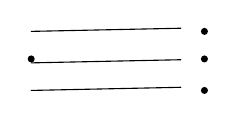
\begin{tikzpicture}[x=1mm,y=1mm,line cap=round,line join=round,font=\scriptsize]
\draw (45,-18.5) -- (64,-18.1);
\draw (45,-22.5) -- (64,-22.1);
\draw (45,-26) -- (64,-25.6);
\node[pt] at (67,-18.5) {};
\node[pt] at (67,-22) {};
\node[pt] at (67,-26) {};
\node[pt] at (45,-22) {};
\end{tikzpicture}
\end{document}
